% Thanks to http://tex.stackexchange.com/a/30782/5645 for this
% example!
\documentclass{article}
\usepackage{amsmath}
\usepackage{ amssymb}
\usepackage{mathptmx}
\usepackage{tikz}
\usepackage{pgfplots}
\usepgfplotslibrary{polar}
\usepgfplotslibrary{fillbetween}
\usepackage{tkz-fct}
\usetikzlibrary{angles, quotes}
\usetikzlibrary{arrows.meta, arrows}
\usetikzlibrary{shapes.geometric}
\usetikzlibrary{external}
\tikzexternalize[prefix={external/}]

\tikzset{
    export as png/.style={
        external/system call/.add={}{
            && convert -density #1 -transparent white "\image.pdf" "\image.png"
        },
    },
    export as png/.default={200},
    % Arrow tips
    >=stealth,
}

% pgfplots settings
\input{colors}
\input{pgfplots}

\DeclareSymbolFont{symbolsb}{OMS}{cmsy}{m}{n}
\SetSymbolFont{symbolsb}{bold}{OMS}{cmsy}{b}{n}
\DeclareSymbolFontAlphabet{\mathcal}{symbolsb}

\def\req{\protect\rotatebox{90}{$\scriptstyle=$}}

\newcommand{\addaxes}{\draw (0em,1em) -- (0em,-1em)
                            (-1em,0em) -- (1em,0em);}
\newcommand{\stepfunc}{\draw[line width=1.5pt] (0.65em,0.65em) -- (0,0.65em) 
                                    -- (0,-0.65em) -- (-0.65em,-0.65em);}

\begin{document}

\tikzset{export as png}

\tikzsetnextfilename{funcion-biyectiva}

% Author: Alfredo Sánchez Alberca (asalber@ceu.es)
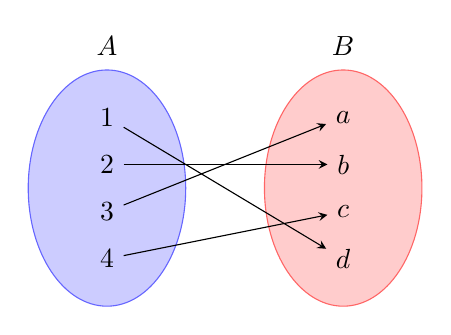
\begin{tikzpicture}[scale=1,every node/.style={transform shape}]
    \filldraw[fill=blue!20, draw=blue!60] (-1.5,0) ellipse (1cm and 1.5cm);
    \filldraw[fill=red!20, draw=red!60] (1.5,0) ellipse (1cm and 1.5cm);
    
        \node at (-1.5,1.8) {$A$};
        \node at (1.5,1.8) {$B$};
    
        \node (x1) at (-1.5,0.9) {$1$};
        \node (x2) at (-1.5,0.3) {$2$};
        \node (x3) at (-1.5,-0.3) {$3$};
        \node (x4) at (-1.5,-0.9) {$4$};
        \node (y1) at (1.5,0.9) {$a$};
        \node (y2) at (1.5,0.3) {$b$};
        \node (y3) at (1.5,-0.3) {$c$};
        \node (y4) at (1.5,-0.9) {$d$};
    
        % draw the arrows
        \draw[-stealth] (x1) -- (y4);
        \draw[-stealth] (x2) -- (y2);
        \draw[-stealth] (x3) -- (y1);
        \draw[-stealth] (x4) -- (y3);
    
    \end{tikzpicture}

\end{document}